
\lstinputlisting[language=bash,basicstyle=\small]{python_codes/fieldstone_21/keywords}

\begin{center}
Code at \url{https://github.com/cedrict/fieldstone/tree/master/python_codes/fieldstone_21}
\end{center}

\par\noindent\rule{\textwidth}{0.4pt}

{\sl This benchmark was developed in collaboration with Prof. E.G.P. Puckett}. 
\index{contributors}{E.G.P. Puckett}

\par\noindent\rule{\textwidth}{0.4pt}
%%%%%%%%%%%%%%%%%%%%%%%%%%%%%%%%%%%%%%%%%%%%%%%%%%%%%%%%%%%%%%%%%%%%%%%%%%%%%%%%%%%%%%%%%%%%

The benchmark is described fully in Stone 9. 
The following results have been obtained with $k=4$.
Taylor-Hood $Q_2\times Q_1$ elements are used with an isoparametric mapping. 

For simplicity the layout of the points is borrowed from Stone 9 which 
showcases $Q_1 \times P_0$ elements. However the points are then 'grouped' 
to form $Q_2$ elements and $Q_1$ elements. 
The used parameters $nelr$ and $nelt$ are read in and then halved. Concretely, 
when the script is ran with $nelr=10$ the real number of $Q_2$ elements 
in the radial direction is then 5. In this stone the number of elements
in the tangential direction is fixed to $nelt=12*nelr$.

In this current version of the code, I have opted not to remove the pressure nullspace
off the matrix and I simply carry out a simple post-processing which consists of 
removing the average pressure as measured on the inner boundary (or outer boundary -- it 
yields the same result) from the pressure fields $p$ and $q$ (the projection of the 
$Q_1$ pressure onto the $Q_2$ mesh). 

Just for a change I here compute the velocity gradient tensor first ${\bm L}(\vec\upnu)=\vec\nabla\vec\upnu$.
I loop over elements. For each element I loop over its velocity nodes and use the $Q_2$ 
shape function derivatives to compute the four components $L_{xx},L_{xy},L_{yx},L_{yy}$ at 
the node and add this value to the node (while keeping track of how many times a value
has been added to the node). In the end I simply compute the average of the values
on each node. From ${\bm L}(\vec\upnu)$ I then compute $\dot{\bm \varepsilon}(\vec\upnu)$. 

As expected we recover a cubic convergence for the velocity error and quadratic for the 
pressure. We also recover nearly identical results as those obtained with ASPECT (note that 
in this case $h=(R_2-R_1)/nelr=1/nelr$): 

\begin{center}
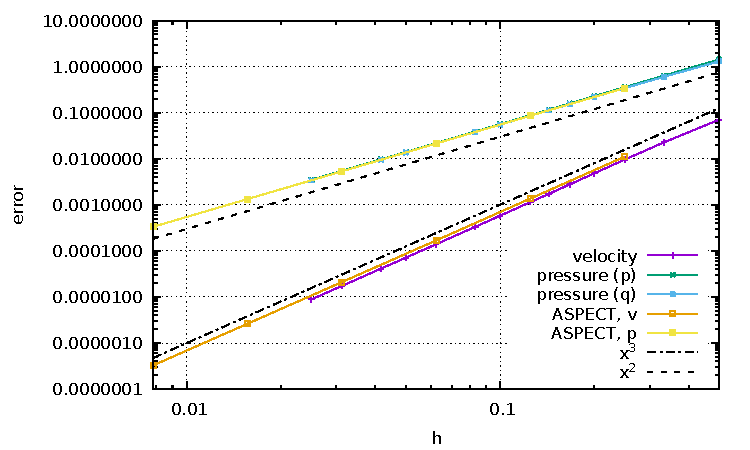
\includegraphics[width=10cm]{python_codes/fieldstone_21/results/errors.pdf}
\end{center}

Also the root mean square velocity is logically found to converge to its 
expected analytical value.

\begin{center}
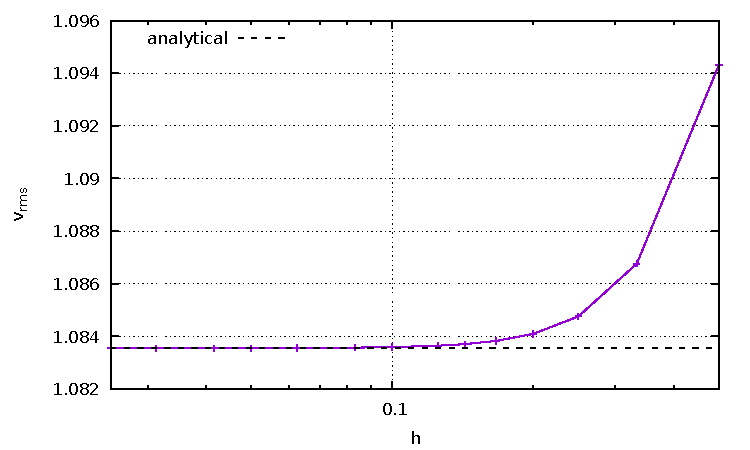
\includegraphics[width=10cm]{python_codes/fieldstone_21/results/vrms.pdf}
\end{center}

The pressure $p$ and its projection onto the $Q_2$ grid at 
$r=R_1$ and $r=R_2$ are plotted here under:

\begin{center}
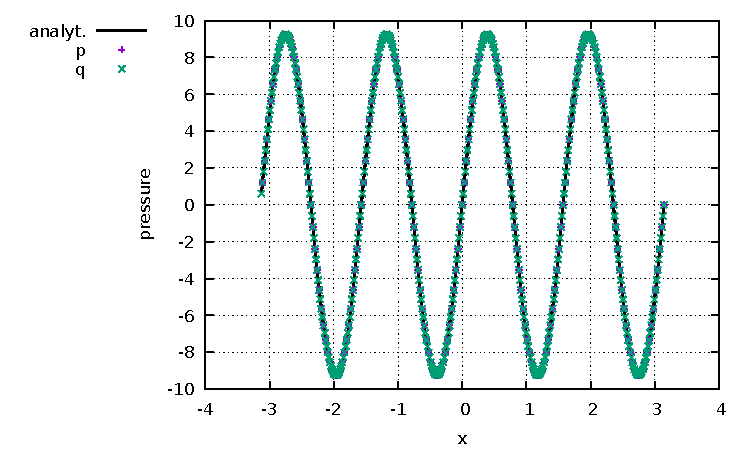
\includegraphics[width=10cm]{python_codes/fieldstone_21/results/pressure_R1.pdf}\\
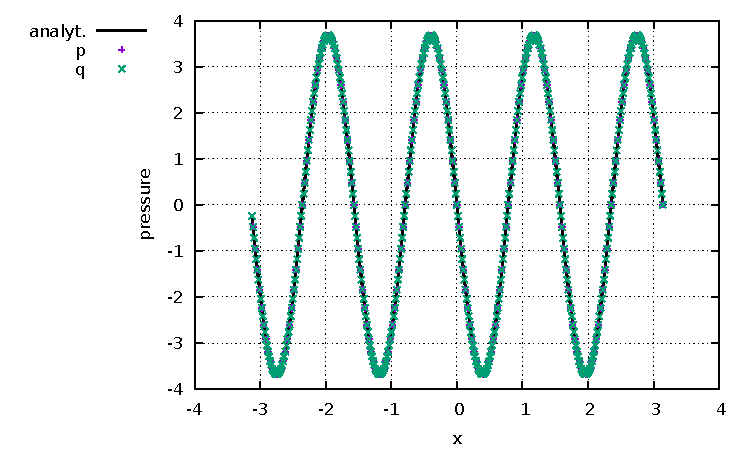
\includegraphics[width=10cm]{python_codes/fieldstone_21/results/pressure_R2.pdf}\\
{\captionfont Left: pressure $p$ and $q$ at $r=R_1$; Right: 
pressure $p$ and $q$ at $r=R_2$.}
\end{center}

\newpage
\begin{center}
a)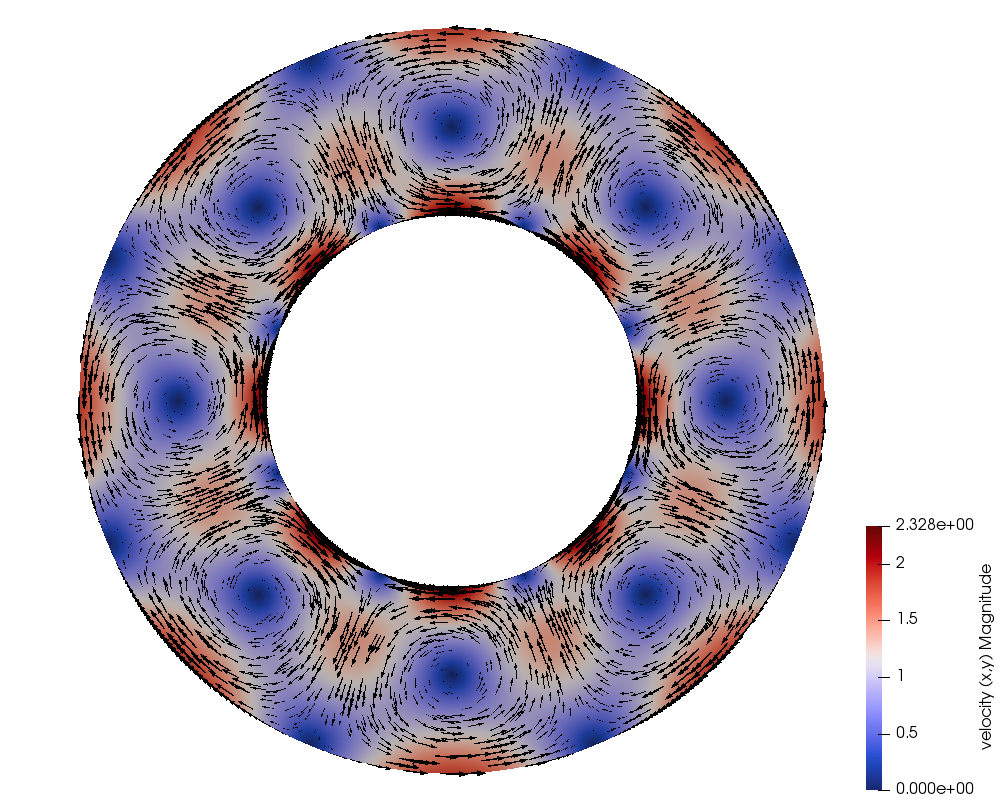
\includegraphics[width=7.3cm]{python_codes/fieldstone_21/results/vel}
b)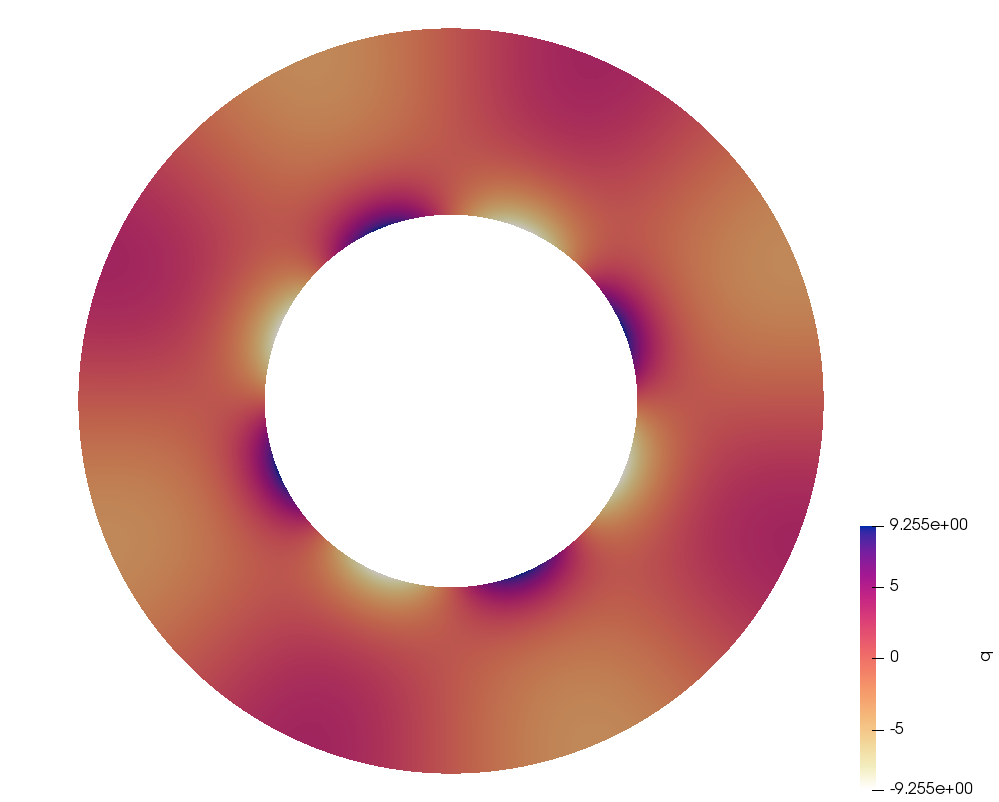
\includegraphics[width=7.3cm]{python_codes/fieldstone_21/results/q}\\
c)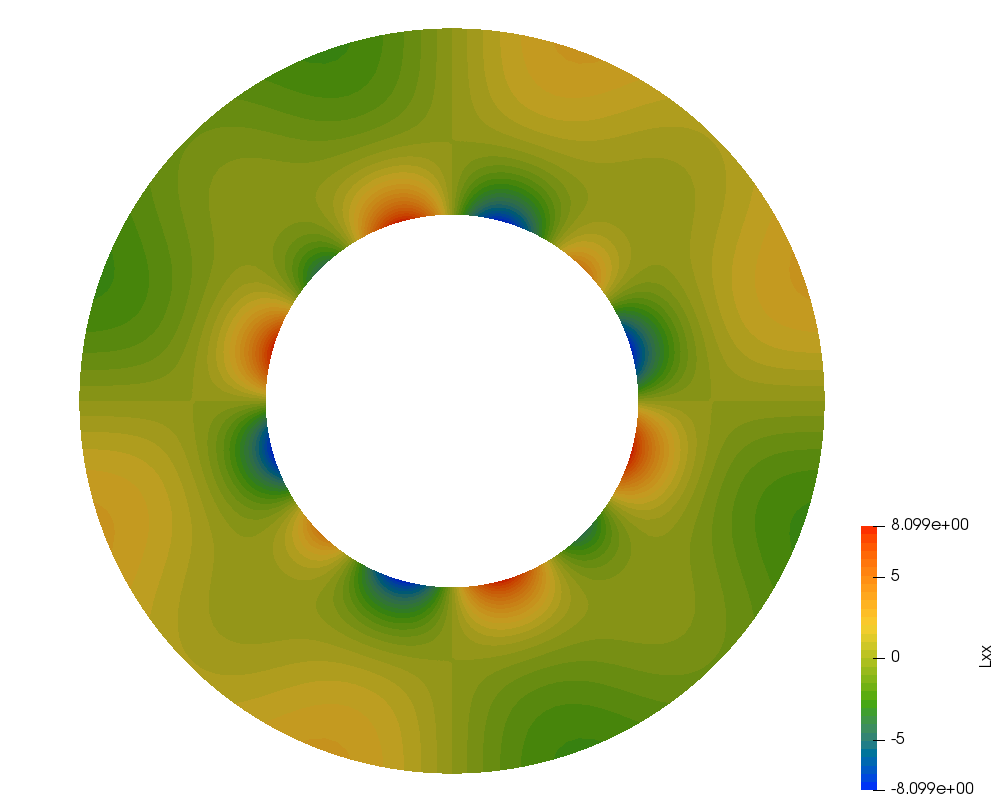
\includegraphics[width=7.3cm]{python_codes/fieldstone_21/results/Lxx}
d)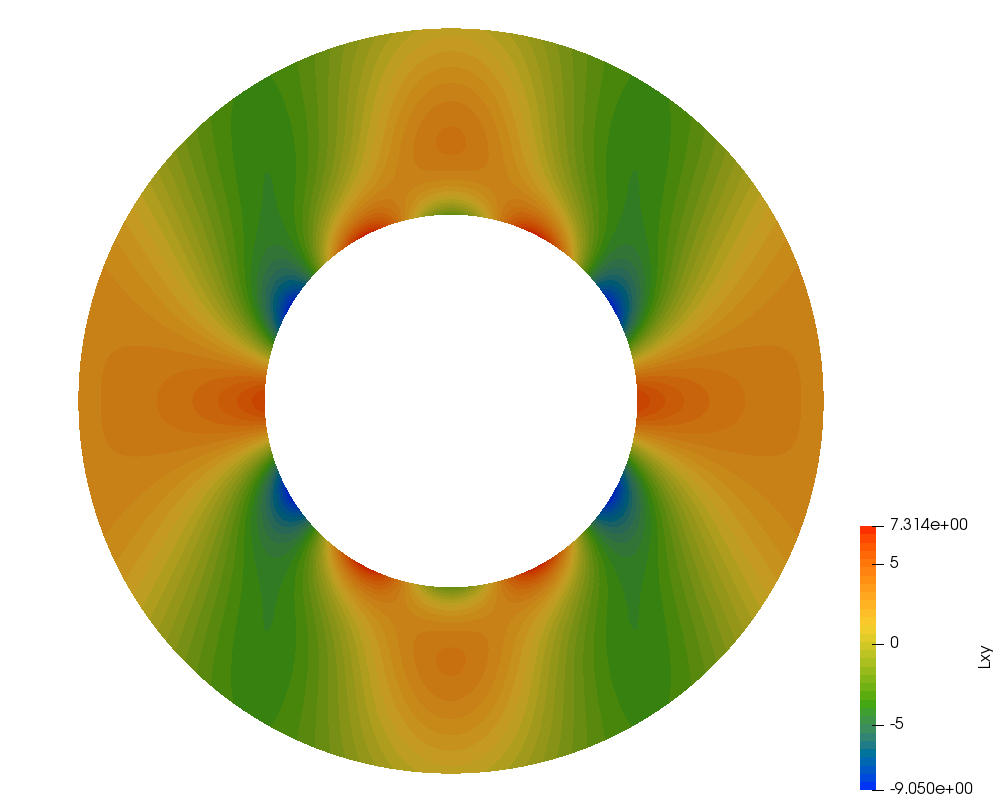
\includegraphics[width=7.3cm]{python_codes/fieldstone_21/results/Lxy}\\
e)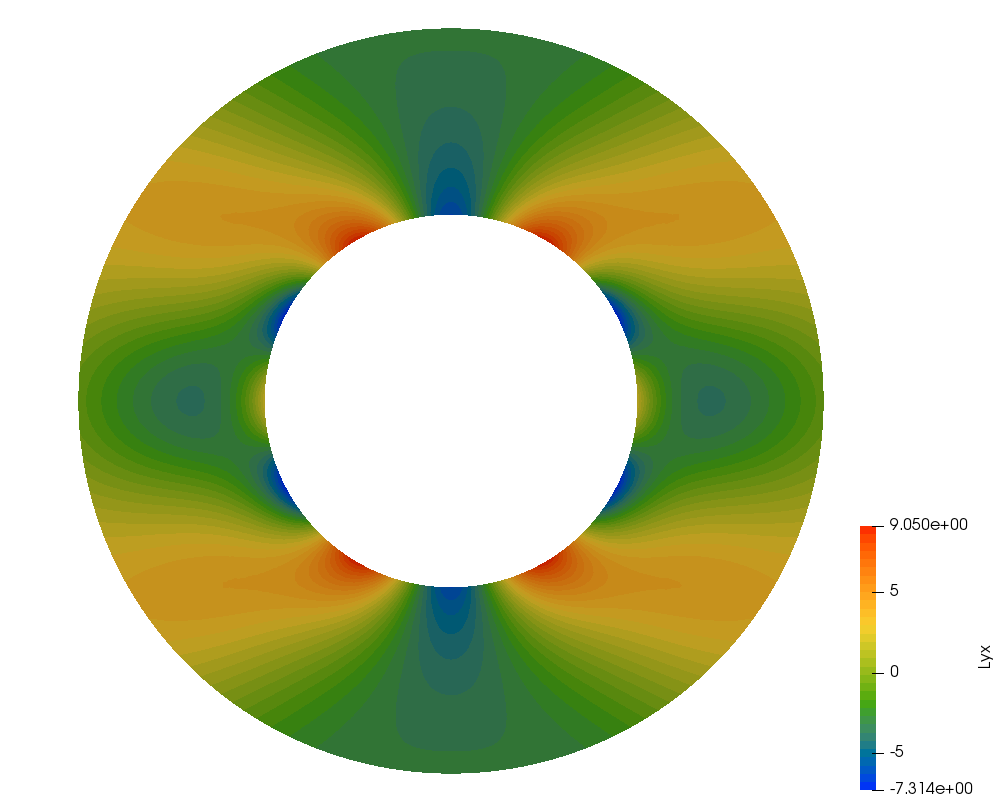
\includegraphics[width=7.3cm]{python_codes/fieldstone_21/results/Lyx}
f)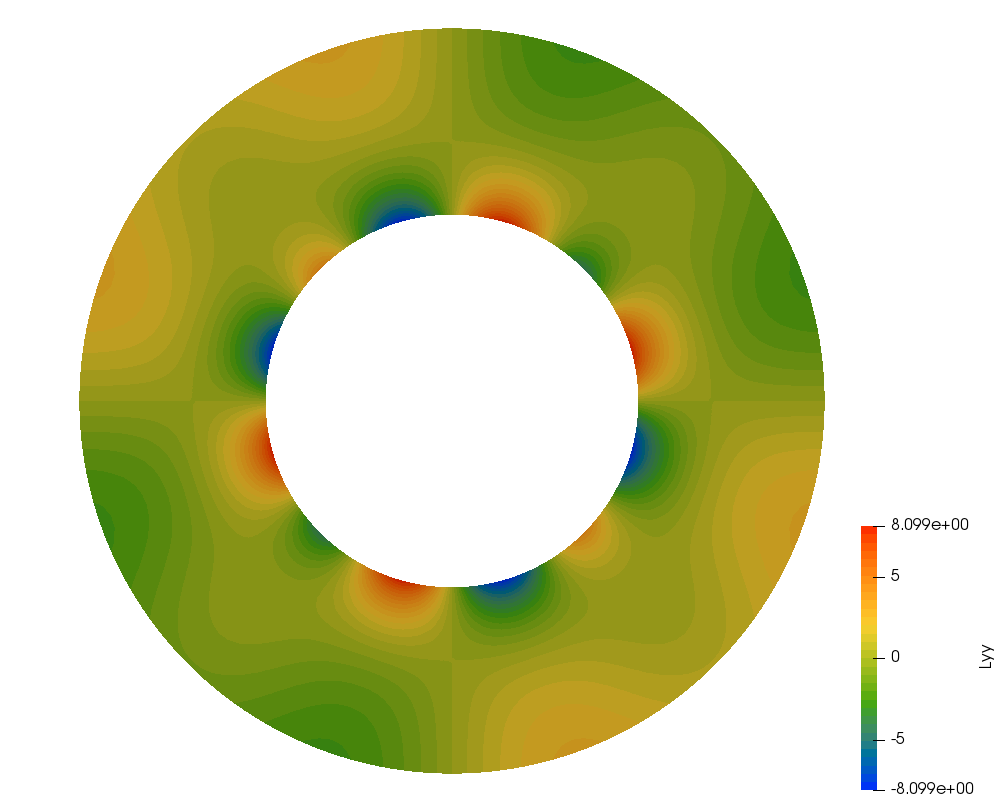
\includegraphics[width=7.3cm]{python_codes/fieldstone_21/results/Lyy}\\
{\captionfont a) velocity field; b) pressure; 
c) $L_{xx}$; 
d) $L_{xy}$; 
e) $L_{yx}$; 
f) $L_{yy}$.}
\end{center}
